\chapter{Data Collection}
For the extended project, eight participants tested the prototype (five males, three females; average age 23).

Figures \ref{fig:1}, \ref{fig:2}, \ref{fig:3}, \ref{fig:4}, \ref{fig:5}, \ref{fig:6}, \ref{fig:7}, \ref{fig:8}, \ref{fig:9} show the results from the tests. Since the test also included other elements in the questionnaire (such as collecting data on demographics, emotions, and specific questions about the gameplay), not all of the questions mentioned in Section \ref{qustionnaire} have been included.

\begin{figure}[htbp]
\centering
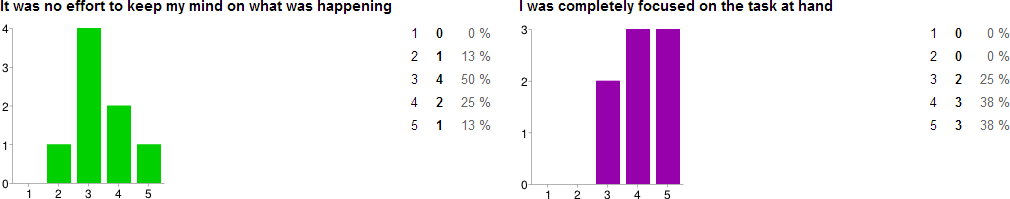
\includegraphics[width=1.0\textwidth]{Pictures/flow_1_focus}
\caption{Data}
\label{fig:1}
\end{figure}

\begin{figure}[htbp]
\centering
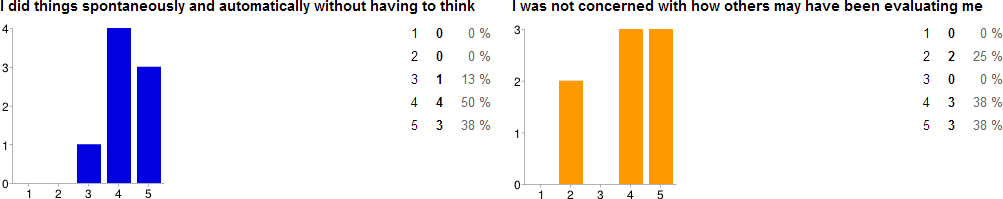
\includegraphics[width=1.0\textwidth]{Pictures/flow_2_social}
\caption{Data}
\label{fig:2}
\end{figure}

\begin{figure}[htbp]
\centering
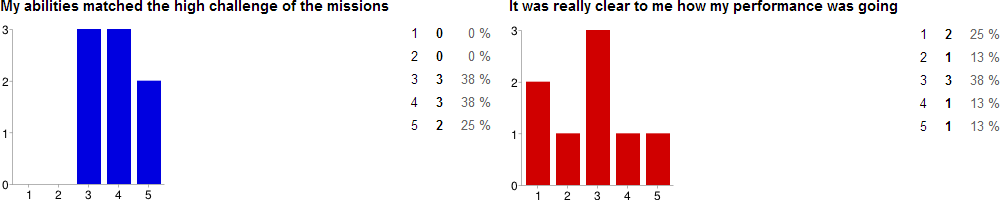
\includegraphics[width=1.0\textwidth]{Pictures/flow_3_senseOfControl}
\caption{Data}
\label{fig:3}
\end{figure}

\begin{figure}[htbp]
\centering
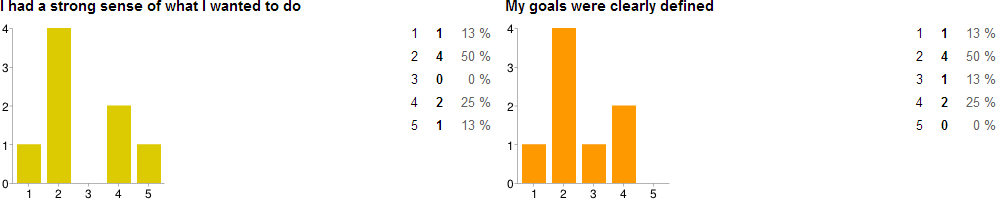
\includegraphics[width=1.0\textwidth]{Pictures/flow_4_senseOfControl}
\caption{Data}
\label{fig:4}
\end{figure}

\begin{figure}[htbp]
\centering
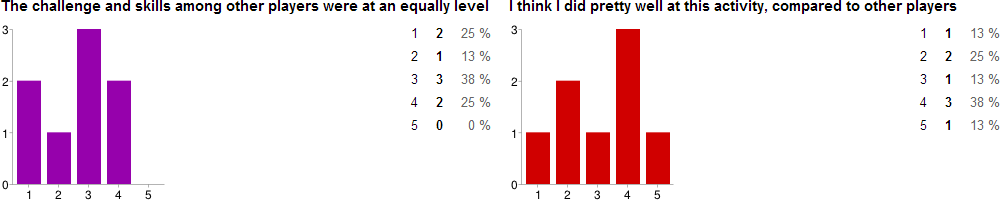
\includegraphics[width=1.0\textwidth]{Pictures/flow_5_senseOfControl}
\caption{Data}
\label{fig:5}
\end{figure}

\begin{figure}[htbp]
\centering
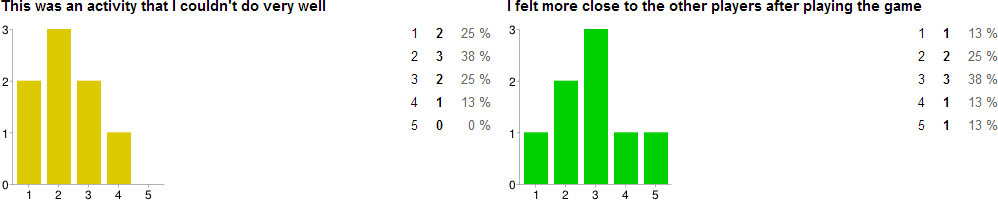
\includegraphics[width=1.0\textwidth]{Pictures/imi_1}
\caption{Data}
\label{fig:6}
\end{figure}

\begin{figure}[htbp]
\centering
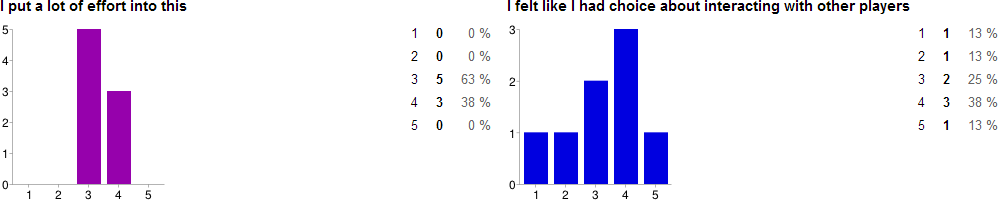
\includegraphics[width=1.0\textwidth]{Pictures/imi_2}
\caption{Data}
\label{fig:7}
\end{figure}

\begin{figure}[htbp]
\centering
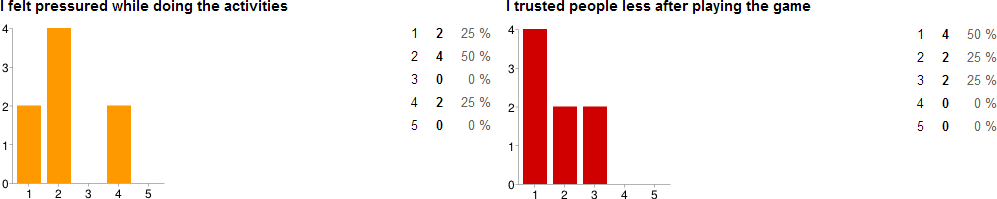
\includegraphics[width=1.0\textwidth]{Pictures/imi_3}
\caption{Data}
\label{fig:8}
\end{figure}

\begin{figure}[htbp]
\centering
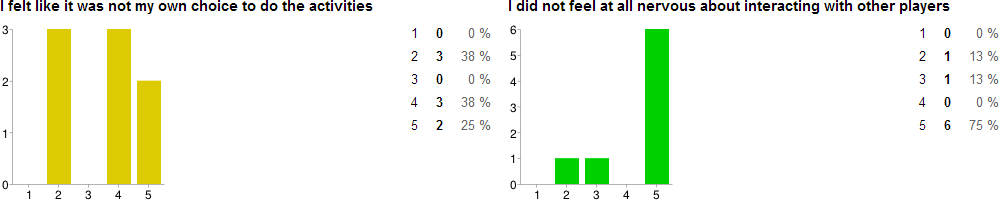
\includegraphics[width=1.0\textwidth]{Pictures/imi_4}
\caption{Data}
\label{fig:9}
\end{figure}